\documentclass[dvipdfmx]{jsarticle}
\setcounter{section}{2}
\setcounter{subsection}{7}
\usepackage{xr}
\externaldocument{1.2.5}
\usepackage{amsmath,amsfonts,amssymb,array,comment,mathtools,url,docmute}
\usepackage{longtable,booktabs,dcolumn,tabularx,mathtools,multirow,colortbl,xcolor}
\usepackage[dvipdfmx]{graphics}
\usepackage{bmpsize}
\usepackage{amsthm}
\usepackage{enumitem}
\setlistdepth{20}
\renewlist{itemize}{itemize}{20}
\setlist[itemize]{label=•}
\renewlist{enumerate}{enumerate}{20}
\setlist[enumerate]{label=\arabic*.}
\setcounter{MaxMatrixCols}{20}
\setcounter{tocdepth}{3}
\newcommand{\rotin}{\text{\rotatebox[origin=c]{90}{$\in $}}}
\newcommand{\amap}[6]{\text{\raisebox{-0.7cm}{\begin{tikzpicture} 
  \node (a) at (0, 1) {$\textstyle{#2}$};
  \node (b) at (#6, 1) {$\textstyle{#3}$};
  \node (c) at (0, 0) {$\textstyle{#4}$};
  \node (d) at (#6, 0) {$\textstyle{#5}$};
  \node (x) at (0, 0.5) {$\rotin $};
  \node (x) at (#6, 0.5) {$\rotin $};
  \draw[->] (a) to node[xshift=0pt, yshift=7pt] {$\textstyle{\scriptstyle{#1}}$} (b);
  \draw[|->] (c) to node[xshift=0pt, yshift=7pt] {$\textstyle{\scriptstyle{#1}}$} (d);
\end{tikzpicture}}}}
\newcommand{\twomaps}[9]{\text{\raisebox{-0.7cm}{\begin{tikzpicture} 
  \node (a) at (0, 1) {$\textstyle{#3}$};
  \node (b) at (#9, 1) {$\textstyle{#4}$};
  \node (c) at (#9+#9, 1) {$\textstyle{#5}$};
  \node (d) at (0, 0) {$\textstyle{#6}$};
  \node (e) at (#9, 0) {$\textstyle{#7}$};
  \node (f) at (#9+#9, 0) {$\textstyle{#8}$};
  \node (x) at (0, 0.5) {$\rotin $};
  \node (x) at (#9, 0.5) {$\rotin $};
  \node (x) at (#9+#9, 0.5) {$\rotin $};
  \draw[->] (a) to node[xshift=0pt, yshift=7pt] {$\textstyle{\scriptstyle{#1}}$} (b);
  \draw[|->] (d) to node[xshift=0pt, yshift=7pt] {$\textstyle{\scriptstyle{#2}}$} (e);
  \draw[->] (b) to node[xshift=0pt, yshift=7pt] {$\textstyle{\scriptstyle{#1}}$} (c);
  \draw[|->] (e) to node[xshift=0pt, yshift=7pt] {$\textstyle{\scriptstyle{#2}}$} (f);
\end{tikzpicture}}}}
\renewcommand{\thesection}{第\arabic{section}部}
\renewcommand{\thesubsection}{\arabic{section}.\arabic{subsection}}
\renewcommand{\thesubsubsection}{\arabic{section}.\arabic{subsection}.\arabic{subsubsection}}
\everymath{\displaystyle}
\allowdisplaybreaks[4]
\usepackage{vtable}
\theoremstyle{definition}
\newtheorem{thm}{定理}[subsection]
\newtheorem*{thm*}{定理}
\newtheorem{dfn}{定義}[subsection]
\newtheorem*{dfn*}{定義}
\newtheorem{axs}[dfn]{公理}
\newtheorem*{axs*}{公理}
\renewcommand{\headfont}{\bfseries}
\makeatletter
  \renewcommand{\section}{%
    \@startsection{section}{1}{\z@}%
    {\Cvs}{\Cvs}%
    {\normalfont\huge\headfont\raggedright}}
\makeatother
\makeatletter
  \renewcommand{\subsection}{%
    \@startsection{subsection}{2}{\z@}%
    {0.5\Cvs}{0.5\Cvs}%
    {\normalfont\LARGE\headfont\raggedright}}
\makeatother
\makeatletter
  \renewcommand{\subsubsection}{%
    \@startsection{subsubsection}{3}{\z@}%
    {0.4\Cvs}{0.4\Cvs}%
    {\normalfont\Large\headfont\raggedright}}
\makeatother
\makeatletter
\renewenvironment{proof}[1][\proofname]{\par
  \pushQED{\qed}%
  \normalfont \topsep6\p@\@plus6\p@\relax
  \trivlist
  \item\relax
  {
  #1\@addpunct{.}}\hspace\labelsep\ignorespaces
}{%
  \popQED\endtrivlist\@endpefalse
}
\makeatother
\renewcommand{\proofname}{\textbf{証明}}
\usepackage{tikz,graphics}
\usepackage[dvipdfmx]{hyperref}
\usepackage{pxjahyper}
\hypersetup{
 setpagesize=false,
 bookmarks=true,
 bookmarksdepth=tocdepth,
 bookmarksnumbered=true,
 colorlinks=false,
 pdftitle={},
 pdfsubject={},
 pdfauthor={},
 pdfkeywords={}}
\begin{document}
%\hypertarget{ux6fc3ux5ea6}{%
\subsection{濃度}%\label{ux6fc3ux5ea6}}
%\hypertarget{ux96c6ux5408ux306eux5bfeux7b49}{%
\subsubsection{集合の対等}%\label{ux96c6ux5408ux306eux5bfeux7b49}}
\begin{dfn}
2つの集合たち$A$、$B$が与えられたとき、$\exists f \in \mathfrak{F}(A,B)$に対し、その写像$f$が全単射なとき、集合$B$は集合$A$に対等である、集合$A$と集合$B$とは互いに対等であるといい、$A \sim B$、$A \approx B$などと書く。なお、空集合$\emptyset$はただそれ自身のみ対等であるとする。
\end{dfn}
\begin{thm}\label{1.2.7.1}
これについて次のことが成り立つ、即ち、その関係$\sim$は同値関係となる\footnote{実はまずいことがあって集合全体の集合は正則性の公理により存在できないんですよね…。これを回避するのにいろいろな工夫がありますが、これを述べるとかなり長くなるので、申し訳ないのですが、ここでは、省かせていただきます…。当面の間では集合全体の集合ほど大きくないものの十分大きい集合$\mathcal{F}$で考えることにいたしましょう。}。
\begin{itemize}
\item
  $A \sim A$が成り立つ。
\item
  $A \sim B$が成り立つなら、$B \sim A$が成り立つ。
\item
  $A \sim B$かつ$B \sim C$が成り立つなら、$A \sim C$が成り立つ。
\end{itemize}
\end{thm}
\begin{proof}
集合$B$は集合$A$に対等である$A \sim B$とき、集合$A$上の恒等写像$I_{A}$を考えれば、明らかに$A \sim A$が成り立つ。また、$A \sim B$が成り立つなら、$\exists f \in \mathfrak{F}(A,B)$に対し、$f:A\overset{\sim}{\rightarrow}B$が成り立つことになり、$\exists f^{- 1}\in \mathfrak{F}(B,A)$に対し、$f^{- 1}:B\overset{\sim}{\rightarrow}A$が成り立つので、$B \sim A$が成り立つ。最後に、$A \sim B$かつ$B \sim C$が成り立つなら、$\exists f \in \mathfrak{F}(A,B)$に対し、$f:A\overset{\sim}{\rightarrow}B$が成り立つかつ、$\exists g\in \mathfrak{F}(B,C)$に対し、$g:B\overset{\sim}{\rightarrow}C$が成り立つことになり、$h = g \circ f$とすれば、$h:A\overset{\sim}{\rightarrow}B$が成り立つので、$A \sim C$が成り立つ。
\end{proof}
%\hypertarget{bernsteinux306eux5b9aux7406}{%
\subsubsection{Bernsteinの定理}%\label{bernsteinux306eux5b9aux7406}}
\begin{thm}[Bernsteinの定理]\label{1.2.7.2}
2つの集合たち$A$、$B$が存在するとき、次のことは同値である。
\begin{itemize}
\item
  $\exists A'\in \mathfrak{P}(A)$に対し、$A' \sim B$が成り立つかつ、$\exists B'\in \mathfrak{P}(B)$に対し、$A \sim B'$が成り立つ。
\item
  $\exists f\in \mathfrak{F}(A,B)\exists g \in \mathfrak{F}(B,A)$に対し、これらの写像たちがいづれも単射である。
\item
  $A \sim B$が成り立つ。
\end{itemize}\par
\end{thm}\par
この定理はBernsteinの定理といわれる。この定理は次の定理と組み合わせて用いられることが多い。
\begin{thm*}[定理\ref{1.2.5.5}の再掲]
2つの集合たち$A$、$B$が与えられたとする。その集合$A$からその集合$B$への単射が存在するならそのときに限り、その集合$B$からその集合$A$への全射が存在する。
\end{thm*}\par
Bernsteinの定理は次のようにして示される。
\begin{enumerate}
\item
  終集合をいじることで次式を示す。
\begin{align*}
&\quad \exists A'\in \mathfrak{P}(A)\left[ A' \sim B \right] \land \exists B'\in \mathfrak{P}(B)\left[ A \sim B' \right] \\
&\Leftrightarrow \exists f\in \mathfrak{F}(A,B)[ f:A \rightarrowtail B] \land \exists g\in \mathfrak{F}(B,A)[ g:B \rightarrowtail A]
\end{align*}
\item
  上の条件を満たすとき、$f:A \twoheadrightarrow B \Rightarrow A \sim B$を示す。これは直ちに示される。
\item
  $\neg(f:A \twoheadrightarrow B)$のとき、次のように定義する。
\begin{align*}
B_{0} = B \setminus V\left( f|A \right),\ \ \left\{ \begin{matrix}
A_{n + 1} & = & V\left( g|B_{n} \right) \\
B_{n} & = & V\left( f|A_{n} \right) \\
\end{matrix} \right.\ ,\ \ \left\{ \begin{matrix}
A_{*} & = & \bigcup_{n \in \mathbb{N}} A_{n} \\
A^{*} & = & A \setminus A_{*} \\
B_{*} & = & \bigcup_{n \in \mathbb{N} \cup \left\{ 0 \right\}} B_{n} \\
B^{*} & = & B \setminus B_{*} \\
\end{matrix} \right.\ 
\end{align*}
\item
  $V\left( f|A \setminus A_{*} \right) = V(f) \setminus V\left( f|A_{*} \right)$を背理法で示す。
\item
  $\left( B \setminus B_{0} \right) \setminus V\left( f|A_{*} \right) = B \setminus \left( B_{0} \cup V\left( f|A_{*} \right) \right)$を元が属する関係と論理式を用いて示す。
\item
  $B \setminus \left( B_{0} \cup V\left( f|A_{*} \right) \right) = B^{*}$を3.の式々を用いて示す。
\item
  $V\left( g|B_{*} \right) = A_{*}$を3.の式々を用いて示す。
\item
  次式のように定義される写像$h$が全単射であることを示すことで$A \sim B$を示す。
\begin{align*}
h:A \rightarrow B;a \mapsto \left\{ \begin{matrix}
f|A_{*} & {\mathrm {if}} & a \in A^{*} \\
\left( g|B_{*} \right)^{- 1} & {\mathrm {if}} & a \notin A^{*} \\
\end{matrix} \right.\ 
\end{align*}
\item
  最後に$\exists f\in \mathfrak{F}(A,B)[ f:A \rightarrowtail B] \land \exists g \in \mathfrak{F}(B,A)[ g:B \rightarrowtail A] \Leftarrow A \sim B$を示すことで示すべきことは示される。
\end{enumerate}
\begin{proof}
2つの集合たち$A$、$B$が存在し、$\exists A'\in \mathfrak{P}(A)\exists B'\in \mathfrak{P}(B)$に対し、$A' \sim B$かつ$A \sim B'$が成り立つとする。このとき、次のようになる。
\begin{align*}
&\quad \exists A'\in \mathfrak{P}(A)\left[ A' \sim B \right] \land \exists B'\in \mathfrak{P}(B)\left[ A \sim B' \right]\\
&\Leftrightarrow \exists A'\in \mathfrak{P}(A)\exists\varphi\in \mathfrak{F}\left( A',B \right)\left[ \varphi:A'\overset{\sim}{\rightarrow}B \right] \land \exists B'\in \mathfrak{P}(B)\exists\psi \in \mathfrak{F}\left( A,B' \right)\left[ \psi:A\overset{\sim}{\rightarrow}B' \right]\\
&\Leftrightarrow \exists A'\in \mathfrak{P}(A)\exists\varphi^{- 1}\in \mathfrak{F}\left( B,A' \right)\left[ \varphi^{- 1}:B\overset{\sim}{\rightarrow}A' \right] \land \exists B'\in \mathfrak{P}(B)\exists\psi \in \mathfrak{F}\left( A,B' \right)\left[ \psi:A\overset{\sim}{\rightarrow}B' \right]
\end{align*}
ここで、これらの2つの写像たち$\varphi^{- 1}$、$\psi$の終集合をそれぞれ$A$、$B$に変えた写像たちをそれぞれ$g$、$f$とおくと、次のようになる。
\begin{align*}
&\quad \exists A'\in \mathfrak{P}(A)\left[ A' \sim B \right] \land \exists B'\in \mathfrak{P}(B)\left[ A \sim B' \right]\\
&\Rightarrow \exists B'\in \mathfrak{P}(B)\exists f \in \mathfrak{F}(A,B)[ f:A \rightarrowtail B] \\
&\quad \land \exists A'\in \mathfrak{P}(A)\exists g \in \mathfrak{F}(B,A)[ g:B \rightarrowtail A]\\
&\Leftrightarrow \exists f \in \mathfrak{F}(A,B)[ f:A \rightarrowtail B] \land \exists g \in \mathfrak{F}(B,A)[ g:B \rightarrowtail A]
\end{align*}\par
逆に、$\exists f \in \mathfrak{F}(A,B)\exists g \in \mathfrak{F}(B,A)$に対し、これらの写像たちがいづれも単射であるなら、それらの終集合たちをそれぞれ$B' = V(f)$、$A' = V(g)$とした写像たちそれぞれ$\varphi$、$\psi$を考えれば、次のようになり、
\begin{align*}
&\quad \exists f \in \mathfrak{F}(A,B)[ f:A \rightarrowtail B] \land \exists g \in \mathfrak{F}(B,A)[ g:B \rightarrowtail A]\\
&\Rightarrow \exists B'\in \mathfrak{P}(B)\exists\varphi \in \mathfrak{F}\left( A,B' \right)\left[ \varphi:A\overset{\sim}{\rightarrow}B' \right] \\
&\quad \land \exists A'\in \mathfrak{P}(A)\exists\psi\in \mathfrak{F}\left( B,A' \right)\left[ \psi:B\overset{\sim}{\rightarrow}A' \right]\\
&\Leftrightarrow \exists B'\in \mathfrak{P}(B)\exists\varphi \in \mathfrak{F}\left( A,B' \right)\left[ \varphi:A\overset{\sim}{\rightarrow}B' \right] \\
&\quad \land \exists A'\in \mathfrak{P}(A)\exists\psi^{- 1}\in \mathfrak{F}\left( A',B \right)\left[ \psi^{- 1}:A'\overset{\sim}{\rightarrow}B \right]\\
&\Leftrightarrow \exists B'\in \mathfrak{P}(B)\left[ A \sim B' \right] \land \exists A'\in \mathfrak{P}(A)\left[ A' \sim B \right]
\end{align*}
よって、$\exists A'\in \mathfrak{P}(A)\exists B'\in \mathfrak{P}(B)$に対し、$A' \sim B$かつ$A \sim B'$が成り立つ。\par
2つの集合たち$A$、$B$が与えられたとき、$\exists f\in \mathfrak{F}(A,B)\exists g \in \mathfrak{F}(B,A)$に対し、これらの写像たちがいづれも単射であるとする。$f:A \twoheadrightarrow B$なら、$\exists h\in \mathfrak{F}(A,B)$に対し、$h:A\overset{\sim}{\rightarrow}B$が成り立ち明らかに$A \sim B$である。$\neg(f:A \twoheadrightarrow B)$が成り立つなら、$V(f) \neq B$であり集合$B \setminus V\left( f|A \right)$を$B_{0}$として、次式のように定め、
\begin{align*}
\left\{ \begin{matrix}
A_{n + 1} = V\left( g|B_{n} \right) \\
B_{n} = V\left( f|A_{n} \right) \\
\end{matrix} \right.\ 
\end{align*}
これを用いて4つの集合たち$A_{*}$、$A^{*}$、$B_{*}$、$B^{*}$を次式のように定める。
\begin{align*}
A_{*} = \bigcup_{n \in \mathbb{N}} A_{n},A^{*} = A \setminus A_{*},\ \ B_{*} = \bigcup_{n \in \mathbb{N} \cup \left\{ 0 \right\}} B_{n},B^{*} = B \setminus B_{*}
\end{align*}
このとき、次式が成り立つ。
\begin{align*}
V\left( f|A^{*} \right) &= V\left( f|A \setminus A_{*} \right) \\ 
&\supseteq V(f) \setminus V\left( f|A_{*} \right)
\end{align*}
$b \in V(f) \setminus V\left( f|A_{*} \right)$とし、$b \notin V\left( f|A \setminus A_{*} \right)$が成り立つと仮定すると、写像$f$は単射であるから、$\exists!a \in A\left[ b = f(a) \right]$となる。ここで、$a \in A \land a \notin A \setminus A_{*}$なら、次のようになることから、
\begin{align*}
a \in A \land a \notin A \setminus A_{*} &\Leftrightarrow a \in A \land \neg\left( a \in A \land a \notin A_{*} \right)\\
&\Leftrightarrow a \in A \land \left( a \notin A \vee a \in A_{*} \right)\\
&\Leftrightarrow a \in A \land a \in A_{*} \Leftrightarrow a \in A_{*}
\end{align*}
したがって、$a \in A_{*}$となり$b = f(a) \in V\left( f|A_{*} \right)$が成り立つが、これは仮定$b \in V(f) \setminus V\left( f|A_{*} \right)$に矛盾する。したがって、$b \in V\left( f|A \setminus A_{*} \right)$となり$V\left( f|A \setminus A_{*} \right) \subseteq V(f) \setminus V\left( \left. \ f \right|_{A_{*}} \right)$が成り立つ。したがって、次のようになる。
\begin{align*}
V\left( f|A_{*} \right) &= V\left( f|A \setminus A_{*} \right)\\
&= V(f) \setminus V\left( f|A_{*} \right)\\
&= V\left( f|A \right) \setminus V\left( f|A_{*} \right)\\
&= \left( B \setminus B_{0} \right) \setminus V\left( f|A_{*} \right)\ \because\ B_{0} = B \setminus V\left( f|A \right)
\end{align*}
ここで、$b' \in V(f|A_{*})$とすると、次のようになる。
\begin{align*}
&\quad b' \in V\left( f|A^{*} \right) = \left( B \setminus B_{0} \right) \setminus V\left( f|A_{*} \right)\\
&\Leftrightarrow \left( b' \in B \land b' \notin B_{0} \right) \land b' \notin V\left( f|A_{*} \right)\\
&\Leftrightarrow b' \in B \land \left( \neg\left( b' \in B_{0} \right) \land \neg\left( b' \in V\left( f|A_{*} \right) \right) \right)\\
&\Leftrightarrow b' \in B \land \neg\left( b' \in B_{0} \vee b' \in V\left( f|A_{*} \right) \right)\\
&\Leftrightarrow b' \in B \setminus \left( B_{0} \cup V\left( f|A_{*} \right) \right)\\
&\Leftrightarrow b' \in B \setminus \left( B_{0} \cup V\left( f|\bigcup_{n \in \mathbb{N}} A_{n}\  \right) \right)\ \because\ A_{*} = \bigcup_{n \in \mathbb{N}} A_{n}\\
&\Leftrightarrow b' \in B \setminus \left( B_{0} \cup \bigcup_{n \in \mathbb{N}} {V\left( f|A_{n} \right)} \right)\\
&\Leftrightarrow b' \in B \setminus \left( B_{0} \cup \bigcup_{n \in \mathbb{N}} B_{n} \right)\ \because\ B_{n} = V\left( f|A_{n} \right)\\
&\Leftrightarrow b' \in B \setminus \left( \bigcup_{n \in \mathbb{N} \cup \left\{ 0 \right\}} B_{n} \right)\\
&\Leftrightarrow b' \in B \setminus B_{*} \Leftrightarrow b' \in B^{*}\ \because\ B_{*} = \bigcup_{n \in \mathbb{N} \cup \left\{ 0 \right\}} B_{n}
\end{align*}
したがって、次式が成り立つ。
\begin{align*}
V\left( f|A^{*} \right) = \left( B \setminus B_{0} \right) \setminus V\left( f|A_{*} \right) = B^{*}
\end{align*}
また、$A_{n + 1} = g\left( B_{n} \right)$、$A_{*} = \bigcup_{n \in \mathbb{N}} A_{n}$より次のようになる。
\begin{align*}
V\left( g|B_{*} \right) &= g\left( \bigcup_{n \in \mathbb{N} \cup \left\{ 0 \right\}} B_{n} \right) \\
&= g\left( \bigcup_{n \in \mathbb{N}} B_{n - 1} \right) \\
&= \bigcup_{n \in \mathbb{N}} {g\left( B_{n - 1} \right)} \\
&= \bigcup_{n \in \mathbb{N}} A_{n} = A_{*}
\end{align*}
さて、写像$f|A^{*}:A^{*} \rightarrow B_{*}$とすれば、仮定の$f:A \rightarrowtail B$と上記の$V\left( f|A^{*} \right) = B^{*}$より全単射$f|A^{*}:A^{*}\overset{\sim}{\rightarrow}B_{*}$であり、写像$g|B_{*}:B_{*} \rightarrow A^{*}$とすれば、仮定の$g:B \rightarrowtail A$と上記の$V\left( g|B_{*} \right) = A_{*}$より全単射$g|B_{*}:B_{*} \rightarrow A^{*}$である。したがって、この写像$g|B_{*}$には逆写像$\left( g|B_{*} \right)^{- 1}$が存在し、$\left( g|B_{*} \right)^{- 1}:A^{*} = A \setminus A_{*}\overset{\sim}{\rightarrow}B_{*}$である。そこで写像$h:A \rightarrow B$を次のように定義すると、この写像$h$は全単射$h:A\overset{\sim}{\rightarrow}B$であるから、$A \sim B$である。
\begin{align*}
h:A \rightarrow B;a \mapsto \left\{ \begin{matrix}
f|A^{*} & {\mathrm {if}} & a \in A^{*} \\
\left( g|B_{*} \right)^{- 1} & {\mathrm {if}} & a \notin A^{*} \\
\end{matrix} \right.\ 
\end{align*}\par
逆に、$A \sim B$であるならば、全単射なる写像$f$が存在し、この写像$f$は明らかに$f:A \rightarrowtail B$が成り立つかつ、その写像$f$の逆対応$f^{- 1}$も全単射の写像であるから、明らかに$f^{- 1}:B \rightarrowtail A$が得られる。よって、$\exists f \in \mathfrak{F}(A,B)\exists g \in \mathfrak{F}(B,A)$に対し、これらの写像たちがいづれも単射である。
\end{proof}
%\hypertarget{ux6fc3ux5ea6-1}{%
\subsubsection{濃度}%\label{ux6fc3ux5ea6-1}}
\begin{dfn}
集合の対等関係$\sim$は同値関係であったので、集合が属するような大きい集合$\mathcal{F}$を同値類$\frac{\mathcal{F}}{\sim}$に類別することができ、このようにして類別したときの各同値類を濃度、数学上濃度、基数といい\footnote{コァ~ディネァレァティあるいはパウゥエァ…φ(゜Д゜)?? これは測度論や組合せ論で大活躍するので、勉強すると頼れる道具になることに間違いなし!}、集合$A$が属する同値類を集合$A$の同値類といい、$\# A$、$\\mathrm{card} A$、$|A|$、$\overline{\overline{A}}$、$n(A)$などと書く。
\end{dfn}
\begin{dfn}
これの大小関係を次式のように定義しよう。
\begin{align*}
\# A = \# B &\Leftrightarrow A \sim B\\
\# A \leq \# B &\Leftrightarrow \exists B'\in \mathfrak{P}(B)\left[ A \sim B' \right]\\
\# A < \# B &\Leftrightarrow \# A \leq \# B \land \# A \neq \# B
\end{align*}
\end{dfn}\par
注意点としては、$B' \subset B$が成り立っても、$\# A < \# B$が成り立つとは限らないことと、$A \sim B'$が成り立つならそのときに限り、$\exists f\in \mathfrak{F}\left( A,B' \right)$に対し、$f:A\overset{\sim}{\rightarrow}B' \subseteq B$が成り立つので、終集合を$B$と変えれば、明らかに$\exists g\in \mathfrak{F}(A,B)$に対し、$g:A \rightarrowtail B$が成り立ち、これが成り立つならそのときに限り、定理\ref{1.2.5.5}より$\exists h\in \mathfrak{F}(B,A)$に対し、$h:B \twoheadrightarrow A$も成り立つことが挙げられる。
\begin{thm}\label{1.2.7.3}
上で定義された関係$\leq$は順序関係となる、即ち、3つの濃度たち$\# A$、$\# B$、$\# C$について次のことが成り立つ。
\begin{itemize}
\item
  $\# A \leq \# A$が成り立つ。
\item
  $\# A \leq \# B$かつ$\# B \leq \# A$が成り立つなら、$\# A = \# B$が成り立つ。
\item
  $\# A \leq \# B$かつ$\# B \leq \# C$が成り立つなら、$\# A \leq \# C$が成り立つ。
\end{itemize}
\end{thm}\par
この定理を示すときの注意点として、関係$\leq$は自然数の順序関係とは別に定義されていることが挙げられる。
\begin{proof}
3つの濃度たち$\# A$、$\# B$、$\# C$について考える。\par
恒等写像$I_{A}$は全単射で$A \subseteq A$が成り立つので、$\# A \leq \# A$が成り立つ。\par
$\# A \leq \# B$かつ$\# B \leq \# A$が成り立つならそのときに限り、$\exists A'\in \mathfrak{P}(A)$に対し、$A' \sim B$が成り立つかつ、$\exists B'\in \mathfrak{P}(B)$に対し、$A \sim B'$が成り立つ。Bernsteinの定理より$A \sim B$が成り立つので、濃度の定義より$\# A = \# B$が成り立つ。\par
$\# A \leq \# B$かつ$\# B \leq \# C$が成り立つなら、$\# A \leq \# B \leq \# C$が成り立つなら、$\exists B'\in \mathfrak{P}(B)$に対し、$A \sim B'$が成り立つかつ、$\exists C'\in \mathfrak{P}(C)$に対し、$B \sim C'$が成り立つ。これにより、全単射な写像たち$f:A \rightarrow B'$、$g:B \rightarrow C'$が存在して、これらの写像たちの終集合たちをそれぞれ$B$、$C$とすれば、単射な写像たち$f':A \rightarrowtail B;a \mapsto f(a)$、$g':B \rightarrowtail C;b \mapsto g(b)$が得られる。このとき、その合成写像$g \circ f$も単射であるから、その終集合を$V(g \circ f)$とすれば、写像$h:A \rightarrow V(g \circ f);a \mapsto g \circ f(a)$は全単射である。$V(g \circ f) \subseteq C$なので、濃度の定義より$\# A \leq \# C$が成り立つ。\par
ゆえに、その関係$\leq$は順序関係となる。
\end{proof}
%\hypertarget{ux53efux7b97ux96c6ux5408}{%
\subsubsection{可算集合}%\label{ux53efux7b97ux96c6ux5408}}
\begin{dfn}
集合$\mathbb{N}$の濃度$\# \mathbb{N}$を可算の濃度、可付番の濃度といい$\aleph_{0}$と書く。ある集合$A$について$\# A \leq \aleph_{0}$が成り立つとき、その集合$A$はたかだか可算である、たかだか可算的であるといい、特に、$\# A = \aleph_{0}$が成り立つとき、即ち、集合$\mathbb{N}$と対等であるとき、可算集合、可付番集合という\footnote{カウゥンエァブルセト…φ(. . ) ちなみに濃度がこれより大きい集合となってしまうとその集合の元はまともに自然数でnumberingできなくなってしまうんですよ~。}。任意の可算集合$A$は$A \sim \mathbb{N}$であるので、写像$f:\mathbb{N}\overset{\sim}{\rightarrow}A;n \mapsto a_{n}$より$A = \left\{ a_{n} \right\}_{n \in \mathbb{N}}$と書かれることができ、その写像$f$は数列とみなせることもできる。
\end{dfn}
\begin{dfn}
  集合$\mathbb{R}$の濃度$\# \mathbb{R}$を連続の濃度といい$\aleph$などと書く\footnote{実は$\# \mathbb{N} <\# \mathbb{R}$が成り立つことが知られている。}。
\end{dfn}
\begin{dfn}
  可算の濃度$\aleph_{0}$は$\aleph_{0} = \# \mathbb{N}$と定義されるのであった。ある集合$A$の濃度$\# A$が可算な濃度$\aleph_{0}$に等しいようなその集合$A$を可算集合、可付番集合などと、このとき、その集合$A$は可算である、可付番であるなどという。これはその集合$\mathbb{N}$からその集合$A$への全単射$f$が存在することになり、したがって、その集合$A$の各元$a$は$a = f(n)$となるような自然数$n$が存在できる。
\end{dfn}
\begin{dfn}
  ある集合$A$の濃度$\# A$が可算な濃度$\aleph_{0}$以下になるようなその集合$A$をその集合$A$はたかだか可算であるなどという。
\end{dfn}
\begin{dfn}
  ある集合の濃度がその濃度$\aleph_{0}$より大きいその集合を非可算集合といい、このとき、その集合は非可算であるなどという。
\end{dfn}  
\begin{thm}\label{1.2.7.4}
その集合$\mathbb{N} $と直積$\mathbb{N}^{2}$とは対等である、即ち、$\mathbb{N} \sim \mathbb{N}^{2}$が成り立つ。
\end{thm}
\begin{proof} 次式のように定義される写像$f$を考える。
\begin{align*}
f:\mathbb{N}^{2} \rightarrow \mathbb{N};(m,n) \mapsto 2^{m - 1}(2n - 1)
\end{align*}
このとき、$\forall n \in \mathbb{N}\exists!p \in \mathbb{Z}\exists!q \in \mathbb{N}\left[ 0 \leq p \land \exists m \in \mathbb{N}[ n = 2m - 1] \Rightarrow n = 2^{p}q \right]$が成り立つかつ、$m - 1 \in \mathbb{Z} \land 0 \leq m - 1$が成り立つかつ、$2n - 1 \in \mathbb{N} \land \exists n \in \mathbb{N}[ 2n - 1 = 2n - 1]$が成り立つので、その写像$f$は全単射である。
\end{proof}
%\hypertarget{ux305fux304bux3060ux304bux53efux7b97ux3067ux3042ux308b}{%
\subsubsection{たかだか可算である}%\label{ux305fux304bux3060ux304bux53efux7b97ux3067ux3042ux308b}}
\begin{thm}\label{1.2.7.6}
任意の無限集合$A$は必ず可算集合$B$を部分集合として含む。
\end{thm}
\begin{proof}
1つの集合系$\mathfrak{M}$を定義域としこれの各元$A$において値$A$をとるような写像$\varPhi:\mathfrak{M}\mathfrak{\rightarrow M};A \mapsto A$を$\left( \varPhi_{A} \right)_{A \in \mathfrak{M}}$と書くとすれば、この集合族$\left( \varPhi_{A} \right)_{A \in \mathfrak{M}}$をその集合系$\mathfrak{M}$から自明に定まる集合族ということにし、$\varPhi_{A} = \varPhi(A) = A$が成り立つので、$(A)_{A \in \mathfrak{M}}$とも書くことにする。ここで、1つの無限集合$A$の空集合を除く部分集合系$\mathfrak{P}(A) \setminus \emptyset$を$\mathfrak{M}$とおくと、その集合族$(A)_{A \in \mathfrak{M}}$は空集合でない集合たちからなる集合族であるから、選択の公理より$\forall A \in \mathfrak{M}$に対して$a_{A} = a(A) \in A$となるような元の族$\left( a_{A} \right)_{A \in \mathfrak{M}}$が存在できる。このような元の族を1つ定めておき帰納的に次式のように写像$\left( a_{i} \right)_{i \in \varLambda_{n}}$を定めると、
\begin{align*}
\left( a_{i} \right)_{i \in \varLambda_{n}}:\varLambda_{n} \rightarrow A;n \mapsto a_{n} = \left\{ \begin{matrix}
a_{A} & {\mathrm {if}} & n = 1 \\
a_{A \setminus \left\{ a_{i} \right\}_{i \in \varLambda_{n}}} & {\mathrm {if}} & n \geq 2 \\
\end{matrix} \right.\ 
\end{align*}
この写像$\left( a_{i} \right)_{i \in \varLambda_{n}}$の値域$\left\{ a_{i} \right\}_{i \in \varLambda_{n}}$はその集合の可算な部分集合である。
\end{proof}
\begin{thm}\label{1.2.7.7}
たかだか可算な集合について次のことが成り立つ。
\begin{itemize}
\item
  たかだか可算な集合たち$A$、$B$の直積$A \times B$もたかだか可算である。
\item
  2つの集合たち$A$、$B$がいづれも空集合でなくたかだか可算であり、これらの集合たちの少なくともどちらかが可算なら、直積$A \times B$は可算である。
\item
  空集合でないたかだか可算な添数集合$\varLambda$を用いてある集合族$\left( A_{\lambda} \right)_{\lambda \in \varLambda}$において、$\forall\lambda \in \varLambda$に対し、それらの集合たち$A_{\lambda}$がたかだか可算であるなら、その和集合$\bigcup_{\lambda \in \varLambda} A_{\lambda}$もたかだか可算である。
\item
  空集合でないたかだか可算な添数集合$\varLambda$を用いてある集合族$\left( A_{\lambda} \right)_{\lambda \in \varLambda}$において、$\forall\lambda \in \varLambda$に対し、それらの集合たち$A_{\lambda}$が空集合でなくたかだか可算であるかつ、$\exists\lambda \in \varLambda$に対し$A_{\lambda}$が可算であるなら、その和集合$\bigcup_{\lambda \in \varLambda} A_{\lambda}$は可算である。
\end{itemize}
\end{thm}
\begin{proof}
たかだか可算な集合たち$A$、$B$について、2つの単射たち$f:A \rightarrowtail \mathbb{N}$、$g:B \rightarrowtail \mathbb{N}$が存在し、写像$\varphi$が$\varphi:A \times B \rightarrow \mathbb{N}^{2};(a,b) \mapsto \left( f(a),f(b) \right)$と定義されれば、その写像$\varphi$も単射であり$\# (A \times B) \leq \# \mathbb{N}^{2} = \# \mathbb{N} = \aleph_{0}$が得られる。よって、その直積$A \times B$もたかだか可算である。\par
特に、2つの集合たち$A$、$B$がいづれも空集合でなくたかだか可算であり、これらの集合たちの少なくともどちらかが可算なら、その集合$A$が可算である場合、$b \in B$なる元$b$を取り出せば、写像$f:A \times \left\{ b \right\} \rightarrow A$は明らかに全単射であるから、$A \times \left\{ b \right\} \sim A$が成り立つかつ、$A \times \left\{ b \right\} \subseteq A \times B$が成り立つので、$\# \left( A \times \left\{ b \right\} \right) = \# \mathbb{N} = \aleph_{0}$が成り立つかつ、$\# \left( A \times \left\{ b \right\} \right) \leq \# (A \times B)$が成り立つ。ここで、上記より$\# (A \times B) \leq \aleph_{0}$が成り立つのであったので、$\aleph_{0} = \# \left( A \times \left\{ b \right\} \right) \leq \# (A \times B) \leq \aleph_{0}$が得られ、よって、$\# (A \times B) = \aleph_{0}$が成り立ちその直積$A \times B$は可算である。\par
空集合でないたかだか可算な添数集合$\varLambda$を用いてある集合族$\left( A_{\lambda} \right)_{\lambda \in \varLambda}$において$\forall\lambda \in \varLambda$に対しそれらの集合たち$A_{\lambda}$がたかだか可算であるなら、上記より集合$\varLambda \times \mathbb{N}$は可算である。また、仮定より$\forall\lambda \in \varLambda$に対し$\# A_{\lambda} \leq \# \mathbb{N}$が成り立ち全射$f_{\lambda}:\mathbb{N} \rightarrow A_{\lambda}$が存在する。ここで、次式のように写像$\varphi$を定義すれば、
\begin{align*}
\varphi:\varLambda \times \mathbb{N} \rightarrow \bigcup_{\lambda \in \varLambda} A_{\lambda};(\lambda,n) \mapsto f_{\lambda}(n)
\end{align*}
$\forall a \in \bigcup_{\lambda \in \varLambda} A_{\lambda}\exists\lambda \in \varLambda$に対し$a \in A_{\lambda}$が成り立ち、このような元$\lambda$に対しその写像$f_{\lambda}$は全射であったので、$a = f_{\lambda}(n)$となるその集合$\mathbb{N}$の元$n$が必ず存在する。したがって、その写像$\varphi$は全射となるので、$\# {\bigcup_{\lambda \in \varLambda} A_{\lambda}} \leq \# \left( \varLambda \times \mathbb{N} \right) = \aleph_{0}$が成り立ち、その和集合$\bigcup_{\lambda \in \varLambda} A_{\lambda}$もたかだか可算である。\par
特に、空集合でないたかだか可算な添数集合$\varLambda$を用いてある集合族$\left( A_{\lambda} \right)_{\lambda \in \varLambda}$において、$\forall\lambda \in \varLambda$に対しそれらの集合たち$A_{\lambda}$が空集合でなくたかだか可算であるかつ、$\exists\lambda' \in \varLambda$に対し$A_{\lambda'}$が可算であるなら、$a \in \bigcup_{\lambda \in \varLambda} A_{\lambda}$なる元$a$を取り出せば、写像$f:A_{\lambda'} \times \left\{ a \right\} \rightarrow A_{\lambda'}$は明らかに全単射であるから、$A_{\lambda'} \times \left\{ a \right\} \sim A_{\lambda'}$が成り立つかつ、$A_{\lambda'} \times \left\{ a \right\} \subseteq \bigcup_{\lambda \in \varLambda} A_{\lambda}$が成り立つので、$\# \left( A_{\lambda'} \times \left\{ a \right\} \right) = \# \mathbb{N} = \aleph_{0}$が成り立つかつ、$\# \left( A \times \left\{ b \right\} \right) \leq \# {\bigcup_{\lambda \in \varLambda} A_{\lambda}}$が成り立つ。ここで、上記より$\# {\bigcup_{\lambda \in \varLambda} A_{\lambda}} \leq \aleph_{0}$が成り立つのであったので、$\aleph_{0} = \# \left( A_{\lambda'} \times \left\{ a \right\} \right) \leq \# {\bigcup_{\lambda \in \varLambda} A_{\lambda}} \leq \aleph_{0}$が得られ、よって、$\# {\bigcup_{\lambda \in \varLambda} A_{\lambda}} = \aleph_{0}$が成り立ちその和集合$\bigcup_{\lambda \in \varLambda} A_{\lambda}$は可算である。
\end{proof}
\begin{thm}\label{1.2.7.8}
これの系として集合たち$\mathbb{Z}$、$\mathbb{Q}$はいずれも可算である。このことについて、ここでは、簡単に証明することにする。
\end{thm}
\begin{proof}
写像$f:\mathbb{N} \rightarrow \mathbb{Z};n \mapsto - n$は全単射であるので、集合$\left\{ m \in \mathbb{Z} \middle| \exists n \in \mathbb{N}[ m = - n] \right\}$はその集合$\mathbb{N}$とは対等であるかつ、集合$\left\{ 0 \right\}$もせいぜい可算である。また、次式のようにその集合$\mathbb{Z}$は構成されることができるので\footnote{正直、あんまり自明じゃないよね…(;´Д`)}、
\begin{align*}
\mathbb{Z} = \mathbb{N} \sqcup \left\{ 0 \right\} \sqcup - \mathbb{N},\ \  - \mathbb{N} = \left\{ m \in \mathbb{Z} \middle| \exists n \in \mathbb{N}[ m = - n] \right\}
\end{align*}
上記の定理よりその集合$\mathbb{Z}$も可算である。\par
また、写像$g:\mathbb{Z} \times \mathbb{N} \rightarrow \mathbb{Q};(m,n) \mapsto \frac{m}{n}$は明らかに全射であるので、$\# \mathbb{Q} \leq \# \left( \mathbb{Z} \times \mathbb{N} \right)$が成り立つ。また、その集合$\mathbb{Z}$は可算で上記より$\# \left( \mathbb{Z} \times \mathbb{N} \right) = \aleph_{0}$が成り立つ。もちろん、$\mathbb{N} \subseteq \mathbb{Q}$が成り立ち写像$g':\mathbb{N} \rightarrow \mathbb{Q};n \mapsto n$は単射となるので、$\# \mathbb{N} \leq \# \mathbb{Q}$が成り立つ。以上より、$\# \mathbb{Q} = \# \mathbb{N} = \aleph_{0}$が成り立ちその集合$\mathbb{Q}$も可算である。
\end{proof}
\begin{thm}\label{1.2.7.9}
ある無限集合$A$とあるたかだか可算な集合$B$について次のことが成り立つ。
\begin{itemize}
\item
  ある無限集合$A$と$B \in \mathfrak{P}(A)$なるたかだか可算な集合$B$について、集合$A \setminus B$が無限集合であるなら、その集合$A \setminus B$はその集合$A$と対等である\footnote{定理\ref{1.2.7.8}と定理\ref{1.2.7.9}より無理数全体の集合の濃度は$\# \mathbb{R}$に等しいことになる。}。
\item
  ある無限集合$A$とあるたかだか可算な集合$B$について、集合$A \cup B$が無限集合であるなら、その集合$A \cup B$はその集合$A$と対等である。
\end{itemize}
\end{thm}
\begin{proof}
ある無限集合$A$と$B \in \mathfrak{P}(A)$なるたかだか可算な集合$B$について集合$A \setminus B$が無限集合であるなら、任意の無限集合は必ず可算集合を部分集合として含むのであったので、$C \subseteq A \setminus B$なる可算な集合$C$が存在する。このとき、次のようになるので、
\begin{align*}
A \setminus B \setminus C \cup (B \cup C) &= (A \setminus B \setminus C \cup C) \cup B \\
&= A \setminus B \cup B = A\\
A \setminus B \setminus C \cap (B \cup C) &= (A \setminus B \setminus C \cap B) \cup (A \setminus B \setminus C \cap C) \\
&= \emptyset \cup \emptyset = \emptyset
\end{align*}
$A \setminus B \setminus C \sqcup (B \cup C) = A$が成り立つかつ、次のようになるので、
\begin{align*}
A \setminus B \setminus C \cup C &= A \setminus B\\
A \setminus B \setminus C \cap C &= \emptyset
\end{align*}
より$A \setminus B \setminus C \sqcup C = A \setminus B$が成り立つ。ここで、空集合でないたかだか可算な添数集合$\varLambda$を用いてある集合族$\left( A_{\lambda} \right)_{\lambda \in \varLambda}$において、$\forall\lambda \in \varLambda$に対し、それらの集合たち$A_{\lambda}$が空集合でなくたかだか可算であるかつ、$\exists\lambda \in \varLambda$に対し、$A_{\lambda}$が可算であるなら、その和集合$\bigcup_{\lambda \in \varLambda} A_{\lambda}$は可算であったので、その集合$B \cup C$も可算である。したがって、2つのそれらの集合たち$C$、$B \cup C$の濃度は等しく全単射$f:B \cup C\overset{\sim}{\rightarrow}C$が存在する。ここで、次式のような写像$g$を考えると、
\begin{align*}
g:A \rightarrow A \setminus B;a \mapsto \left\{ \begin{matrix}
a & {\mathrm {if}} & a \in (A \setminus B) \setminus C \\
f(a) & {\mathrm {if}} & a \in B \cup C \\
\end{matrix} \right.\ 
\end{align*}
即ち、次のような写像$g$を考えると、
\begin{center}
  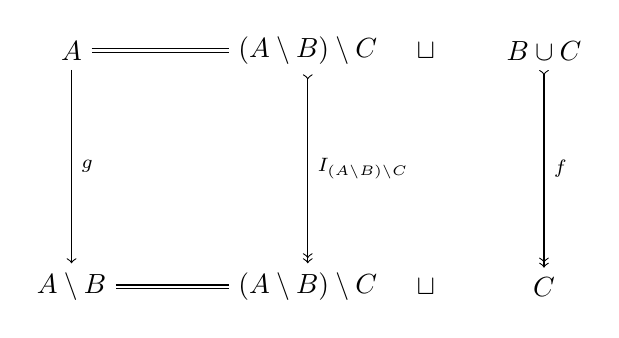
\begin{tikzpicture}[auto] 
    \node (a) at (0, 3) {$A$};
    \node (b) at (3, 3) {$\left( A\setminus B\right) \setminus C$};
    \node (c) at (4.5, 3) {$\sqcup $};
    \node (d) at (6, 3) {$B\cup C$};
    \node (e) at (0, 0) {$A\setminus B$};
    \node (f) at (3, 0) {$\left( A\setminus B\right) \setminus C$};
    \node (g) at (4.5, 0) {$\sqcup $};
    \node (h) at (6, 0) {$C$};
    \draw [->] (a) to node {$\scriptstyle g$} (e);
    \draw [>->>] (b) to node {$\scriptstyle I_{\left( A\setminus B\right) \setminus C}$} (f);
    \draw [>->>] (d) to node {$\scriptstyle f$} (h);
    \draw [double distance=1pt] (a) to node {$\scriptstyle $} (b);
    \draw [double distance=1pt] (e) to node {$\scriptstyle $} (f);
  \end{tikzpicture} 
\end{center}
その終集合$A \setminus B$について、次式が成り立つ、
\begin{center}
  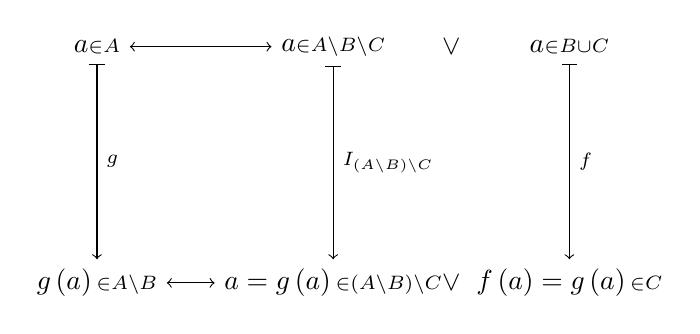
\begin{tikzpicture}[auto] 
    \node (i) at (0, 3) {$a{\scriptstyle\in A} $};
    \node (j) at (3, 3) {$a{\scriptstyle\in A\setminus B\setminus C}$};
    \node (k) at (4.5, 3) {$\vee $};
    \node (l) at (6, 3) {$a{\scriptstyle\in B\cup C}$};
    \node (m) at (0, 0) {$g\left( a\right) {\scriptstyle\in A\setminus B}$};
    \node (n) at (3, 0) {$a=g\left( a\right) {\scriptstyle\in \left( A\setminus B\right) \setminus C}$};
    \node (o) at (4.5, 0) {$\vee $};
    \node (p) at (6, 0) {$f\left( a\right) =g\left( a\right) {\scriptstyle\in C}$};
    \draw [|->] (i) to node {$\scriptstyle g$} (m);
    \draw [|->] (j) to node {$\scriptstyle I_{\left( A\setminus B\right) \setminus C}$} (n);
    \draw [|->] (l) to node {$\scriptstyle f$} (p);
    \draw [<->] (i) to node {$\scriptstyle $} (j);
    \draw [<->] (m) to node {$\scriptstyle $} (n);  
  \end{tikzpicture} 
\end{center}
即ち、$\forall g(a) \in A \setminus B$に対し、$g(a) \in (A \setminus B) \setminus C$または$g(a) \in B \cup C$が成り立つので、$\exists a \in A$に対し、次式が成り立つ。
\begin{align*}
g(a) = \left\{ \begin{matrix}
a & {\mathrm {if}} & a \in (A \setminus B) \setminus C \\
f(a) & {\mathrm {if}} & a \in B \cup C \\
\end{matrix} \right.\ 
\end{align*}
ここで、写像$I_{A}':A \rightarrow A \setminus B;a \mapsto a$が単射であるので、写像$I_{A}'':A \rightarrow (A \setminus B) \setminus C;a \mapsto a$が全単射であるかつ、その写像$f$は全単射であったので、その写像$g$も全単射となる。よって、その集合$A \setminus B$はその集合$A$と対等である。ある無限集合$A$とあるたかだか可算な集合$B$について集合$A \cup B$が無限集合であるなら、集合$(A \cup B) \setminus A$は、次式が成り立つので、
\begin{align*}
(A \cup B) \setminus A = A \setminus A \cup B \setminus A = \emptyset \cup B \setminus A = B \setminus A
\end{align*}
その集合$B$に含まれたかだか可算な集合となる。したがって、ある無限集合$A$と$B \in \mathfrak{P}(A)$なるたかだか可算な集合$B$について$A \setminus B$が無限集合であるなら、その集合$A \setminus B$はその集合$A$と対等であったので、その集合$(A \cup B) \setminus \left( (A \cup B) \setminus A \right)$はその集合$A \cup B$と対等である。また、その集合$(A \cup B) \setminus \left( (A \cup B) \setminus A \right)$を$U$とおくと、次のようになるので、
\begin{align*}
U &= (A \cup B) \setminus \left( (A \cup B) \setminus A \right)\\
&= (A \cup B) \setminus (A \setminus A \cup B \setminus A)\\
&= (A \cup B) \setminus (\emptyset \cup B \setminus A)\\
&= (A \cup B) \setminus \emptyset \cap (A \cup B) \setminus (B \setminus A)\\
&= (A \cup B) \cap (A \cup B) \setminus (B \setminus A)\\
&= (A \cup B) \cap (A \cup B) \cap (A \cup U \setminus B)\\
&= (A \cup B) \cap (A \cup U \setminus B)\\
&= A \cup (B \cap A \setminus B) \\
&= A \cup \emptyset = A
\end{align*}
以上より、よって、その集合$A$はその集合$A \cup B$と対等である。
\end{proof}
%\hypertarget{ux51aaux96c6ux5408ux306eux6fc3ux5ea6}{%
\subsubsection{冪集合の濃度}%\label{ux51aaux96c6ux5408ux306eux6fc3ux5ea6}}
\begin{thm}\label{1.2.7.11}
任意の集合$A$とこれの冪集合$\mathfrak{P}(A)$について、その集合$A$の濃度$\# A$はその集合$\mathfrak{P}(A)の濃度\# {\mathfrak{P}(A)}$より小さい、即ち、$\# A < \# {\mathfrak{P}(A)}$が成り立つ。
\end{thm}\par
これにより、任意の濃度に対してもこれより大きいような濃度が必ず存在できるので、濃度はいくらでも大きいものが存在することができる。
\begin{proof}
任意の集合$A$とこれの冪集合$\mathfrak{P}(A)$について、次式のような写像$f$は明らかに単射である。
\begin{align*}
f:A \rightarrow \mathfrak{P}(A);a \mapsto \left\{ a \right\}
\end{align*}
これにより、$\# A \leq \# {\mathfrak{P}(A)}$が成り立つ。ここで、$\forall g \in \mathfrak{F}\left( A,\mathfrak{P}(A) \right)$に対し、次式のように集合$A'$が与えられたとする。
\begin{align*}
A' = \left\{ a \in A \middle| a \notin g(a) \right\}
\end{align*}
このとき、$\forall a \in A$に対し、その元$a$のその写像$g$による像$g(a)$はその集合$\mathfrak{P}(A)$の元となるので、$a \in A$が成り立つならそのときに限り、$a \in g(a)$または$a \in A \setminus g(a)$が成り立つ。ここで、$a \in g(a)$が成り立つなら、$a \notin A'$が成り立つので、$g(a) \neq A'$が成り立つ。一方で、$a \notin g(a)$が成り立つなら、その集合$A'$の定義より明らかに$a \in A'$が成り立つので、$g(a) \neq A'$が成り立つ。以上より、$\forall a \in A$に対し、$g(a) \neq A'$が成り立つので、次式のようになる。
\begin{align*}
\forall a \in A\left[ A' \notin V\left( g|\left\{ a \right\} \right) \right] &\Leftrightarrow \neg\exists a \in A\left[ A' \in V\left( g \middle| \left\{ a \right\} \right) \right]\\
&\Leftrightarrow \neg A' \in \bigcup_{a \in A} {V\left( g|\left\{ a \right\} \right)}\\
&\Leftrightarrow A' \notin V(g)
\end{align*}
これにより、$V(g)\subset \mathfrak{P}(A)$が成り立つので、その写像$g$は全射であることができない。したがって、$\# A < \# {\mathfrak{P}(A)}$が成り立つ。
\end{proof}
\begin{thebibliography}{50}
  \bibitem{1}
    松坂和夫, 集合・位相入門, 岩波書店, 1968. 新装版第2刷 p61-78 ISBM978-4-00-029871-1
\end{thebibliography}
\end{document}

